\subsection{USB (Universal Serial Bus) \refskript{9.3.9}}
\subsubsection{Electrical characteristics}
\begin{itemize}
	\itemsep-.5em 
	\item Signals are NRZI (non return to zero inverted) encoded
	\item Bit stuffing is used for clock synchronization
\end{itemize}
\begin{center}
	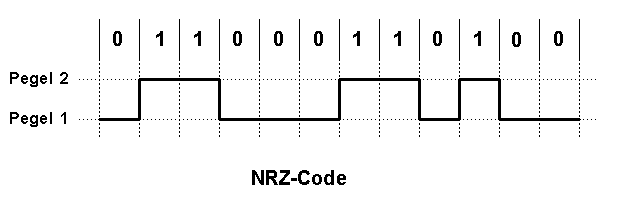
\includegraphics[width=.6\columnwidth]{"Images/NRZ_code.png"}
	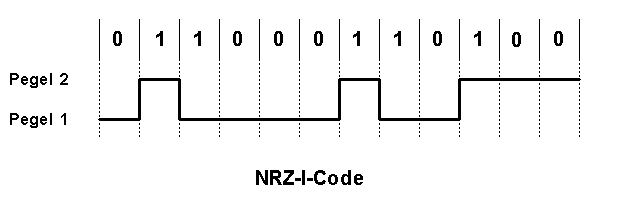
\includegraphics[width=.6\columnwidth]{"Images/NRZI_code.png"}
	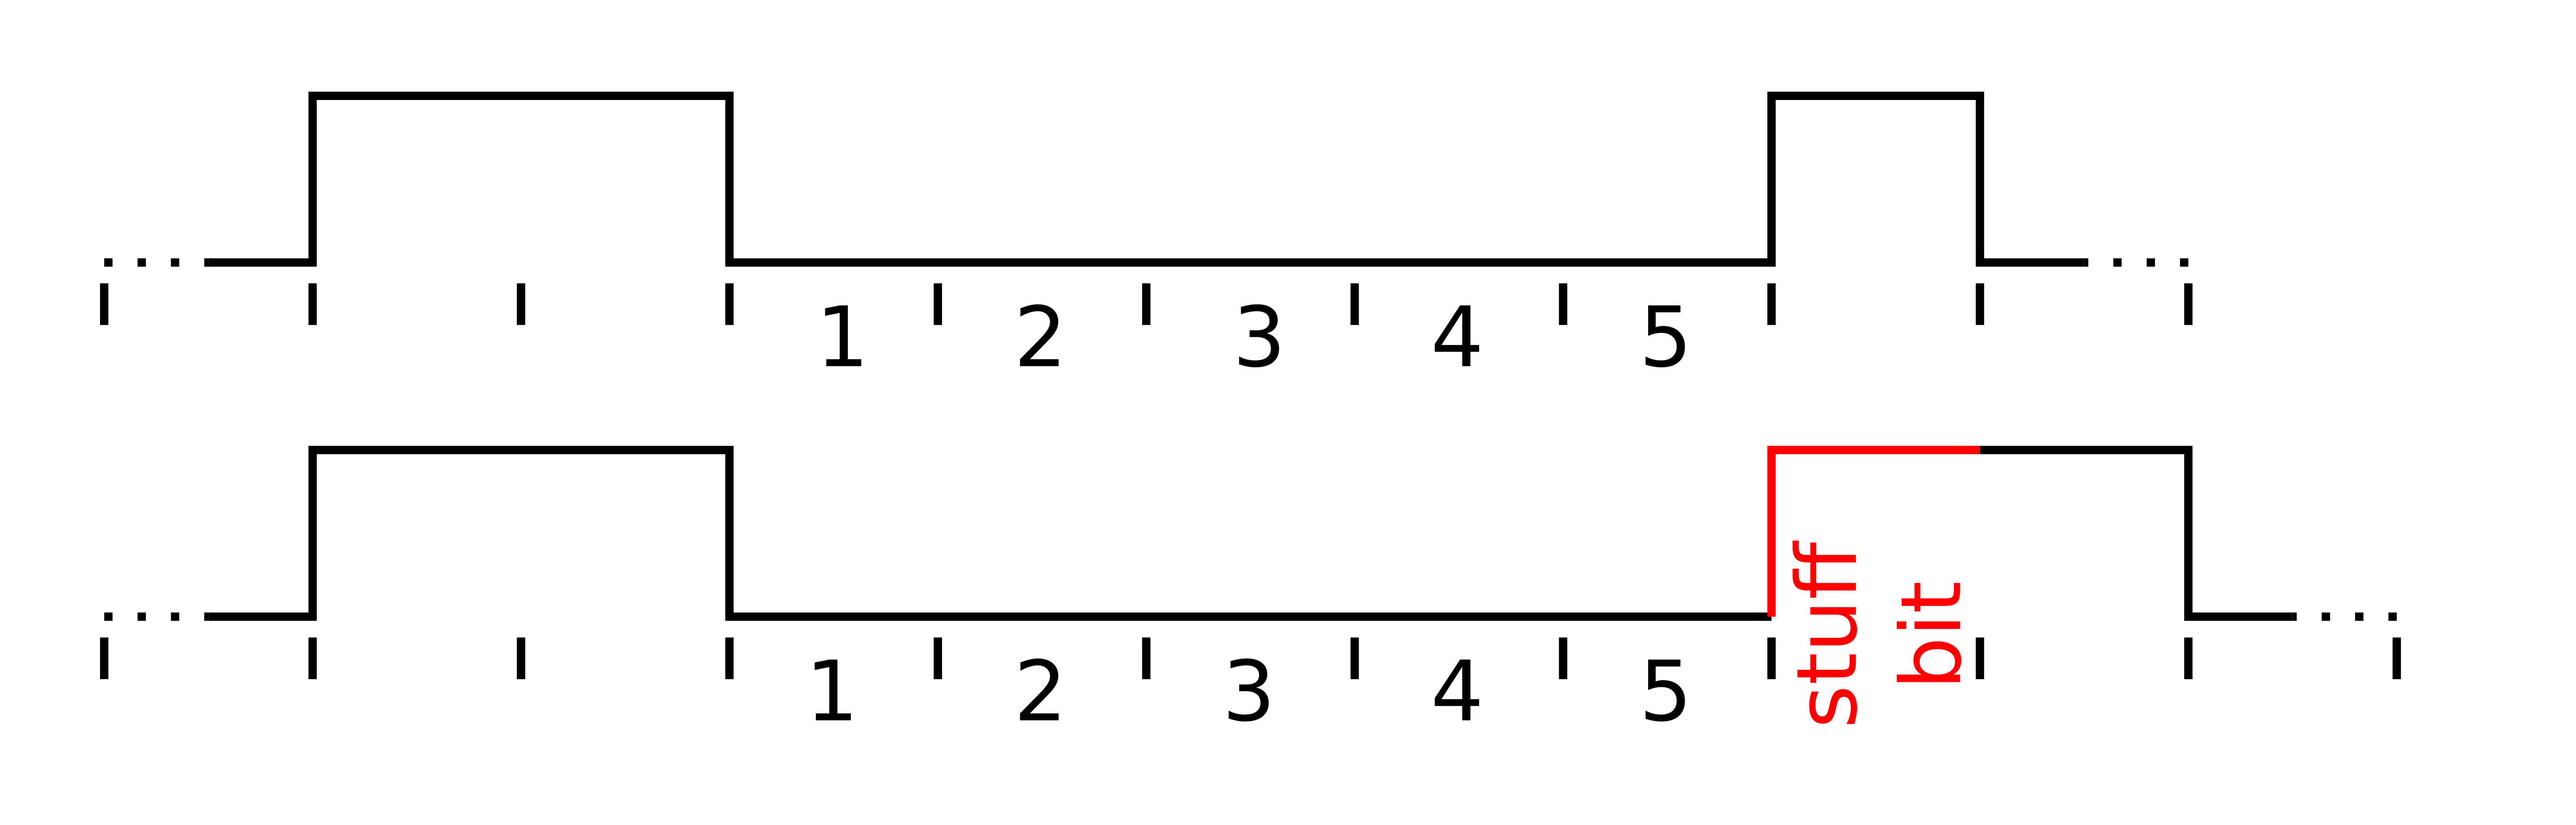
\includegraphics[width=.8\columnwidth]{"Images/BitStuffing.png"}
\end{center}

Each device can have up to total 32 \textbf{endpoints} (16 IN and 16 OUT).
There are different \textbf{packet types}, Token-, Data-, Handshake- and Start of Frame (SOF)- packets which are divided further into \textbf{packet fields} respectively.

There are four Transfer Types / Endpoint Types:
\begin{itemize}
	\itemsep-.5em
	\item Control: Always use of Endpoint 0 (IN \& OUT)
	\item Interrupt: Guaranteed quick responses
	\item Isochronous: Guaranteed data rate, possible data loss
	\item Bulk: Large data transfers using remaining bandwidth
\end{itemize}

USB OTG (On-The-Go) allows to directly connect two OTG capable devices because it can assume the host or the device role.

